\section{Results and Discussion}

\subsection{Results}

In the collection of \textbf{3461} dogs we found, with our method, that they had \textbf{366} variants or alleles of DLA-DRB1. \textbf{769} individuals, or \textbf{0.22\%}, where called homozygotes. \textbf{79} of the alleles had already been found in earlier genotyping projects so \textbf{287} are novel. Of the novel alleles \textbf{25} where found in homozygous individuals. \textbf{179} of the alleles where found in one individual, \textbf{34} in two and \textbf{28} in three individuals. Of the `known' alleles \textbf{35} where not found at all in this dataset.\\ As seen in figure \ref{fig:variants}, \textbf{8} positions had variations that where unique for the reference sequences and \textbf{16} new positions with variation in our data set that have not been seen before. \textbf{54} positions of the \textbf{270} base pair long exon had variation in both the reference alleles and the genotyped dataset.

\begin{figure}[ht]
	\centering
		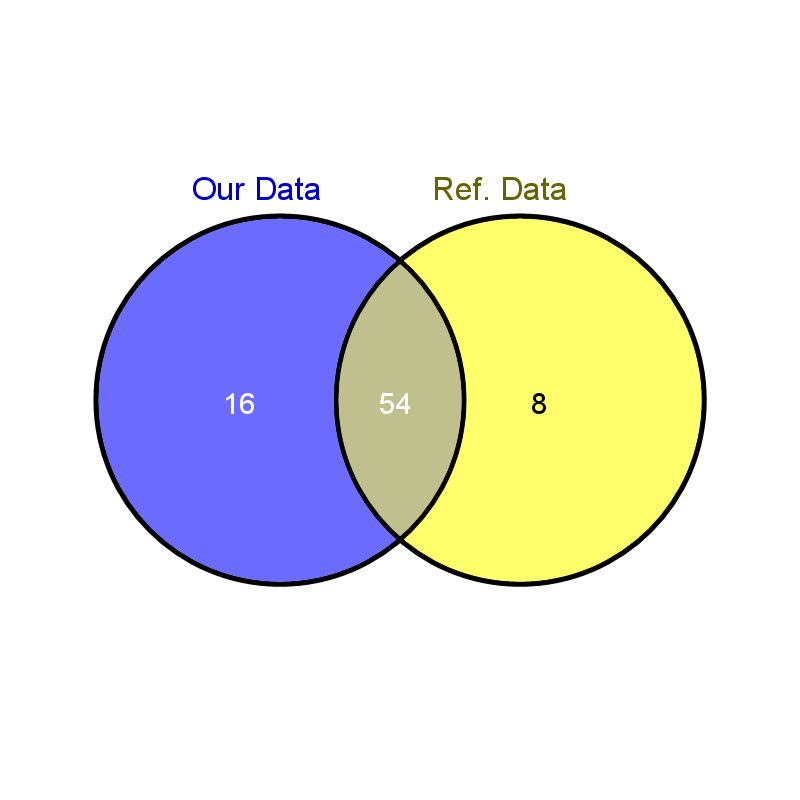
\includegraphics[width=0.6\textwidth]{../pictures/variants.png}
	\caption{Found variants contra reference variants: The figure shows how many variants that the reference sequences and our data set had in common.}
	\label{fig:variants}
\end{figure}


\subsection{Discussion and Conclusions}

When we started to investigate the data we discovered that it was fairly easy to make the alignments by hand. By looking at the sequences we could figure out where it most probably where machine errors contra true variations, or where it should be an insertion or a deletion. Chimeric formations are still hard to detect by eye though. We tried to understand \emph{how} we could tell that the alignments produced by the named softwares are wrong. What made it easier for a human to locate errors than any of the existing algorithms? The conclusion is that we want to incorporate prior knowledge we had about this exon and the sequencing technology into the alignment algorithm, this was how our method was developed.\\

The best way to evaluate the results would have been to compare the variations between different breeds and regions. We would expect to see low variation of alleles within a pure breed, since these stem from a few individuals only. We would also expect to see a greater variation in mixed breeds and the highest diversity in the wolves.\\
Unfortunately the geografic information for the samples are currently missing but if the individuals can be linked to their region of origin in a correct way, the results of this work can help to clarify the origin of dogs. Hopefully this would strengthen any of the hypotheses of dog origin by showing which population that show the highest variety of alleles.\\

Following the earlier discussion about the nature of this exon it is reasonable to belive that some new variable positions is to be seen in a large set of data like this. There is a problem that many of the new alleles were only found in only one individual, it seems unlikely that we see this as often as we do. It is hard to tell how many of these alleles that are false positives based on numbers, but a guess from the initiator of this project was to find about 400 alleles all in all.\\

% Stöd följande påstående med fakta:

Personally i think that the alignment algorithm works fine and do not think that the problems can be traced to this part of the process. Several people have inspected the results of the alignment, and all agree that the algorithm produces the same result as we would have done by hand. The question is how close we can get to reality with such problematic data.\\
